\subsection{Software}
We developed a software package with a user interface that implements the above
linear program and allows configuration of clinicians at [ref \ref{???}], to be
used by the ID division at St. Michael's Hospital. The software was used to
generate the results in the following sections, using real data as well as
simulated data as input. All the following experiments were conducted on an
Intel Core i7-4770k CPU @ 3.50 GHz and 16 GB of RAM running 64-bit Windows 10.
The software was implemented using the COIN-OR Branch-and-Cut open source solver
version 2.9.9 \cite{johnjforrest_coin-or/cbc:_2019}.

\subsection{Infectious Diseases Division}  %main comment  = I think use past
%tense in writing
We used clinician time-off requests and minimum/maximum requirements from
2015-2018 as input data for the ILP problem. Table
\ref{tbl:2018-schedule-comparison} presents the optimal schedule generated using
the software as well as the manually-created schedule for data from 2018. The
schedule is color-coded to distinguish between the different clinicians
assigned. \\

% Table generated by Excel2LaTeX from sheet '2018'
\begin{table}[h]
%	\tiny
 	\centering
 	\begin{adjustbox}{scale=0.8}
	    \begin{tabular}{c||ccc||ccc}
	    	\multicolumn{1}{c||}{\multirow{2}[1]{*}{Week \#}} & \multicolumn{3}{c||}{LP Solution}                                                                                                                                       & \multicolumn{3}{c}{Historical Data}                                                                                                                                     \\
	    	                                                  &                  HIV                  &                                 ID                                 &                              Weekend                               &                  HIV                  &                                 ID                                 &                              Weekend                               \\ \midrule\midrule
	    	                        1                         & \cellcolor[rgb]{ .663,  .816,  .557}A &                \cellcolor[rgb]{ .957,  .69,  .518}E                &                \cellcolor[rgb]{ .957,  .69,  .518}E                & \cellcolor[rgb]{ .663,  .816,  .557}A &                \cellcolor[rgb]{ .957,  .69,  .518}E                &               \cellcolor[rgb]{ .459,  .443,  .443}H                \\
	    	                        2                         & \cellcolor[rgb]{ .663,  .816,  .557}A &                \cellcolor[rgb]{ .957,  .69,  .518}E                &                \cellcolor[rgb]{ .518,  .592,  .69}G                & \cellcolor[rgb]{ .663,  .816,  .557}A &                \cellcolor[rgb]{ .957,  .69,  .518}E                &               \cellcolor[rgb]{ .663,  .816,  .557}A                \\
	    	                        3                         & \cellcolor[rgb]{ .608,  .761,  .902}B &               \cellcolor[rgb]{ .557,  .663,  .859}F                &               \cellcolor[rgb]{ .557,  .663,  .859}F                & \cellcolor[rgb]{ .608,  .761,  .902}B &               \cellcolor[rgb]{ .459,  .443,  .443}H                &                \cellcolor[rgb]{ .518,  .592,  .69}G                \\
	    	                        4                         & \cellcolor[rgb]{ .608,  .761,  .902}B &               \cellcolor[rgb]{ .557,  .663,  .859}F                &               \cellcolor[rgb]{ .459,  .443,  .443}H                & \cellcolor[rgb]{ .608,  .761,  .902}B &               \cellcolor[rgb]{ .459,  .443,  .443}H                & \cellcolor[rgb]{ .251,  .251,  .251}\textcolor[rgb]{ 1,  1,  1}{I} \\
	    	                        5                         & \cellcolor[rgb]{ .663,  .816,  .557}A &                \cellcolor[rgb]{ .518,  .592,  .69}G                &               \cellcolor[rgb]{ .663,  .816,  .557}A                & \cellcolor[rgb]{ .663,  .816,  .557}A &                \cellcolor[rgb]{ .518,  .592,  .69}G                &               \cellcolor[rgb]{ .557,  .663,  .859}F                \\
	    	                        6                         & \cellcolor[rgb]{ .663,  .816,  .557}A &                \cellcolor[rgb]{ .518,  .592,  .69}G                &                \cellcolor[rgb]{ .957,  .69,  .518}E                & \cellcolor[rgb]{ .663,  .816,  .557}A &                \cellcolor[rgb]{ .518,  .592,  .69}G                &                  \cellcolor[rgb]{ 1,  .851,  .4}C                  \\
	    	                        7                         &   \cellcolor[rgb]{ 1,  .851,  .4}C    &               \cellcolor[rgb]{ .608,  .761,  .902}B                &                  \cellcolor[rgb]{ 1,  .851,  .4}C                  & \cellcolor[rgb]{ .663,  .816,  .557}A &               \cellcolor[rgb]{ .557,  .663,  .859}F                &               \cellcolor[rgb]{ .608,  .761,  .902}B                \\
	    	                        8                         &   \cellcolor[rgb]{ 1,  .851,  .4}C    &               \cellcolor[rgb]{ .608,  .761,  .902}B                &                \cellcolor[rgb]{ .518,  .592,  .69}G                & \cellcolor[rgb]{ .788,  .788,  .788}D &                  \cellcolor[rgb]{ 1,  .851,  .4}C                  &                \cellcolor[rgb]{ .518,  .592,  .69}G                \\
	    	                        9                         & \cellcolor[rgb]{ .788,  .788,  .788}D &               \cellcolor[rgb]{ .459,  .443,  .443}H                &               \cellcolor[rgb]{ .788,  .788,  .788}D                & \cellcolor[rgb]{ .608,  .761,  .902}B &                  \cellcolor[rgb]{ 1,  .851,  .4}C                  &               \cellcolor[rgb]{ .788,  .788,  .788}D                \\
	    	                       10                         & \cellcolor[rgb]{ .788,  .788,  .788}D &               \cellcolor[rgb]{ .459,  .443,  .443}H                &               \cellcolor[rgb]{ .459,  .443,  .443}H                & \cellcolor[rgb]{ .608,  .761,  .902}B &               \cellcolor[rgb]{ .788,  .788,  .788}D                &               \cellcolor[rgb]{ .459,  .443,  .443}H                \\
	    	                       11                         & \cellcolor[rgb]{ .663,  .816,  .557}A & \cellcolor[rgb]{ .251,  .251,  .251}\textcolor[rgb]{ 1,  1,  1}{I} & \cellcolor[rgb]{ .251,  .251,  .251}\textcolor[rgb]{ 1,  1,  1}{I} & \cellcolor[rgb]{ .663,  .816,  .557}A &               \cellcolor[rgb]{ .608,  .761,  .902}B                &               \cellcolor[rgb]{ .557,  .663,  .859}F                \\
	    	                       12                         & \cellcolor[rgb]{ .663,  .816,  .557}A & \cellcolor[rgb]{ .251,  .251,  .251}\textcolor[rgb]{ 1,  1,  1}{I} &               \cellcolor[rgb]{ .608,  .761,  .902}B                & \cellcolor[rgb]{ .663,  .816,  .557}A &               \cellcolor[rgb]{ .608,  .761,  .902}B                &               \cellcolor[rgb]{ .663,  .816,  .557}A                \\
	    	                       13                         & \cellcolor[rgb]{ .608,  .761,  .902}B &               \cellcolor[rgb]{ .557,  .663,  .859}F                &               \cellcolor[rgb]{ .557,  .663,  .859}F                &   \cellcolor[rgb]{ 1,  .851,  .4}C    &               \cellcolor[rgb]{ .459,  .443,  .443}H                &               \cellcolor[rgb]{ .459,  .443,  .443}H                \\
	    	                       14                         & \cellcolor[rgb]{ .608,  .761,  .902}B &               \cellcolor[rgb]{ .557,  .663,  .859}F                &               \cellcolor[rgb]{ .459,  .443,  .443}H                &   \cellcolor[rgb]{ 1,  .851,  .4}C    &               \cellcolor[rgb]{ .459,  .443,  .443}H                & \cellcolor[rgb]{ .251,  .251,  .251}\textcolor[rgb]{ 1,  1,  1}{I} \\
	    	                       15                         &   \cellcolor[rgb]{ 1,  .851,  .4}C    & \cellcolor[rgb]{ .251,  .251,  .251}\textcolor[rgb]{ 1,  1,  1}{I} &                  \cellcolor[rgb]{ 1,  .851,  .4}C                  & \cellcolor[rgb]{ .608,  .761,  .902}B & \cellcolor[rgb]{ .251,  .251,  .251}\textcolor[rgb]{ 1,  1,  1}{I} &                  \cellcolor[rgb]{ 1,  .851,  .4}C                  \\
	    	                       16                         &   \cellcolor[rgb]{ 1,  .851,  .4}C    & \cellcolor[rgb]{ .251,  .251,  .251}\textcolor[rgb]{ 1,  1,  1}{I} &               \cellcolor[rgb]{ .663,  .816,  .557}A                & \cellcolor[rgb]{ .608,  .761,  .902}B & \cellcolor[rgb]{ .251,  .251,  .251}\textcolor[rgb]{ 1,  1,  1}{I} &                \cellcolor[rgb]{ .957,  .69,  .518}E                \\
	    	                       17                         & \cellcolor[rgb]{ .608,  .761,  .902}B &               \cellcolor[rgb]{ .788,  .788,  .788}D                &               \cellcolor[rgb]{ .788,  .788,  .788}D                & \cellcolor[rgb]{ .663,  .816,  .557}A &                \cellcolor[rgb]{ .957,  .69,  .518}E                &               \cellcolor[rgb]{ .788,  .788,  .788}D                \\
	    	                       18                         & \cellcolor[rgb]{ .608,  .761,  .902}B &               \cellcolor[rgb]{ .788,  .788,  .788}D                &               \cellcolor[rgb]{ .557,  .663,  .859}F                & \cellcolor[rgb]{ .663,  .816,  .557}A &                \cellcolor[rgb]{ .957,  .69,  .518}E                &                \cellcolor[rgb]{ .957,  .69,  .518}E                \\
	    	                       19                         & \cellcolor[rgb]{ .663,  .816,  .557}A &               \cellcolor[rgb]{ .459,  .443,  .443}H                &               \cellcolor[rgb]{ .459,  .443,  .443}H                & \cellcolor[rgb]{ .663,  .816,  .557}A &                  \cellcolor[rgb]{ 1,  .851,  .4}C                  &               \cellcolor[rgb]{ .557,  .663,  .859}F                \\
	    	                       20                         & \cellcolor[rgb]{ .663,  .816,  .557}A &               \cellcolor[rgb]{ .459,  .443,  .443}H                & \cellcolor[rgb]{ .251,  .251,  .251}\textcolor[rgb]{ 1,  1,  1}{I} & \cellcolor[rgb]{ .663,  .816,  .557}A &                  \cellcolor[rgb]{ 1,  .851,  .4}C                  &                  \cellcolor[rgb]{ 1,  .851,  .4}C                  \\
	    	                       21                         & \cellcolor[rgb]{ .788,  .788,  .788}D &                  \cellcolor[rgb]{ 1,  .851,  .4}C                  &                  \cellcolor[rgb]{ 1,  .851,  .4}C                  & \cellcolor[rgb]{ .608,  .761,  .902}B &                \cellcolor[rgb]{ .518,  .592,  .69}G                &               \cellcolor[rgb]{ .663,  .816,  .557}A                \\
	    	                       22                         & \cellcolor[rgb]{ .788,  .788,  .788}D &                  \cellcolor[rgb]{ 1,  .851,  .4}C                  &                \cellcolor[rgb]{ .518,  .592,  .69}G                & \cellcolor[rgb]{ .608,  .761,  .902}B &                \cellcolor[rgb]{ .518,  .592,  .69}G                &                  \cellcolor[rgb]{ 1,  .851,  .4}C                  \\
	    	                       23                         & \cellcolor[rgb]{ .608,  .761,  .902}B &                \cellcolor[rgb]{ .957,  .69,  .518}E                &                \cellcolor[rgb]{ .957,  .69,  .518}E                &   \cellcolor[rgb]{ 1,  .851,  .4}C    &               \cellcolor[rgb]{ .557,  .663,  .859}F                &               \cellcolor[rgb]{ .788,  .788,  .788}D                \\
	    	                       24                         & \cellcolor[rgb]{ .608,  .761,  .902}B &                \cellcolor[rgb]{ .957,  .69,  .518}E                &               \cellcolor[rgb]{ .557,  .663,  .859}F                &   \cellcolor[rgb]{ 1,  .851,  .4}C    &               \cellcolor[rgb]{ .557,  .663,  .859}F                &                  \cellcolor[rgb]{ 1,  .851,  .4}C                  \\
	    	                       25                         & \cellcolor[rgb]{ .663,  .816,  .557}A &               \cellcolor[rgb]{ .459,  .443,  .443}H                &               \cellcolor[rgb]{ .663,  .816,  .557}A                &   \cellcolor[rgb]{ 1,  .851,  .4}C    &                  \cellcolor[rgb]{ 1,  .851,  .4}C                  &                \cellcolor[rgb]{ .518,  .592,  .69}G                \\
	    	                       26                         & \cellcolor[rgb]{ .663,  .816,  .557}A &               \cellcolor[rgb]{ .459,  .443,  .443}H                &               \cellcolor[rgb]{ .459,  .443,  .443}H                & \cellcolor[rgb]{ .788,  .788,  .788}D & \cellcolor[rgb]{ .251,  .251,  .251}\textcolor[rgb]{ 1,  1,  1}{I} &               \cellcolor[rgb]{ .788,  .788,  .788}D                \\
	    	                       27                         & \cellcolor[rgb]{ .608,  .761,  .902}B &                  \cellcolor[rgb]{ 1,  .851,  .4}C                  &                  \cellcolor[rgb]{ 1,  .851,  .4}C                  & \cellcolor[rgb]{ .663,  .816,  .557}A &               \cellcolor[rgb]{ .608,  .761,  .902}B                &                \cellcolor[rgb]{ .957,  .69,  .518}E                \\
	    	                       28                         & \cellcolor[rgb]{ .608,  .761,  .902}B &                  \cellcolor[rgb]{ 1,  .851,  .4}C                  &                \cellcolor[rgb]{ .957,  .69,  .518}E                & \cellcolor[rgb]{ .663,  .816,  .557}A &               \cellcolor[rgb]{ .608,  .761,  .902}B                & \cellcolor[rgb]{ .251,  .251,  .251}\textcolor[rgb]{ 1,  1,  1}{I} \\
	    	                       29                         & \cellcolor[rgb]{ .663,  .816,  .557}A &                \cellcolor[rgb]{ .518,  .592,  .69}G                &               \cellcolor[rgb]{ .663,  .816,  .557}A                & \cellcolor[rgb]{ .608,  .761,  .902}B &               \cellcolor[rgb]{ .788,  .788,  .788}D                &               \cellcolor[rgb]{ .788,  .788,  .788}D                \\
	    	                       30                         & \cellcolor[rgb]{ .663,  .816,  .557}A &                \cellcolor[rgb]{ .518,  .592,  .69}G                &               \cellcolor[rgb]{ .608,  .761,  .902}B                & \cellcolor[rgb]{ .608,  .761,  .902}B &               \cellcolor[rgb]{ .788,  .788,  .788}D                &               \cellcolor[rgb]{ .663,  .816,  .557}A                \\
	    	                       31                         &   \cellcolor[rgb]{ 1,  .851,  .4}C    &               \cellcolor[rgb]{ .557,  .663,  .859}F                &                  \cellcolor[rgb]{ 1,  .851,  .4}C                  &   \cellcolor[rgb]{ 1,  .851,  .4}C    &               \cellcolor[rgb]{ .557,  .663,  .859}F                &                \cellcolor[rgb]{ .957,  .69,  .518}E                \\
	    	                       32                         &   \cellcolor[rgb]{ 1,  .851,  .4}C    &               \cellcolor[rgb]{ .557,  .663,  .859}F                &                \cellcolor[rgb]{ .957,  .69,  .518}E                &   \cellcolor[rgb]{ 1,  .851,  .4}C    &               \cellcolor[rgb]{ .557,  .663,  .859}F                &               \cellcolor[rgb]{ .557,  .663,  .859}F                \\
	    	                       33                         & \cellcolor[rgb]{ .608,  .761,  .902}B &               \cellcolor[rgb]{ .788,  .788,  .788}D                &               \cellcolor[rgb]{ .788,  .788,  .788}D                & \cellcolor[rgb]{ .608,  .761,  .902}B &               \cellcolor[rgb]{ .557,  .663,  .859}F                & \cellcolor[rgb]{ .251,  .251,  .251}\textcolor[rgb]{ 1,  1,  1}{I} \\
	    	                       34                         & \cellcolor[rgb]{ .608,  .761,  .902}B &               \cellcolor[rgb]{ .788,  .788,  .788}D                &               \cellcolor[rgb]{ .608,  .761,  .902}B                & \cellcolor[rgb]{ .608,  .761,  .902}B & \cellcolor[rgb]{ .251,  .251,  .251}\textcolor[rgb]{ 1,  1,  1}{I} &                  \cellcolor[rgb]{ 1,  .851,  .4}C                  \\
	    	                       35                         & \cellcolor[rgb]{ .663,  .816,  .557}A & \cellcolor[rgb]{ .251,  .251,  .251}\textcolor[rgb]{ 1,  1,  1}{I} & \cellcolor[rgb]{ .251,  .251,  .251}\textcolor[rgb]{ 1,  1,  1}{I} & \cellcolor[rgb]{ .663,  .816,  .557}A &                \cellcolor[rgb]{ .518,  .592,  .69}G                &                \cellcolor[rgb]{ .518,  .592,  .69}G                \\
	    	                       36                         & \cellcolor[rgb]{ .663,  .816,  .557}A & \cellcolor[rgb]{ .251,  .251,  .251}\textcolor[rgb]{ 1,  1,  1}{I} &                \cellcolor[rgb]{ .518,  .592,  .69}G                & \cellcolor[rgb]{ .663,  .816,  .557}A &                \cellcolor[rgb]{ .518,  .592,  .69}G                & \cellcolor[rgb]{ .251,  .251,  .251}\textcolor[rgb]{ 1,  1,  1}{I} \\
	    	                       37                         & \cellcolor[rgb]{ .788,  .788,  .788}D &                \cellcolor[rgb]{ .518,  .592,  .69}G                &               \cellcolor[rgb]{ .788,  .788,  .788}D                & \cellcolor[rgb]{ .788,  .788,  .788}D &                  \cellcolor[rgb]{ 1,  .851,  .4}C                  &               \cellcolor[rgb]{ .663,  .816,  .557}A                \\
	    	                       38                         & \cellcolor[rgb]{ .788,  .788,  .788}D &                \cellcolor[rgb]{ .518,  .592,  .69}G                &               \cellcolor[rgb]{ .557,  .663,  .859}F                & \cellcolor[rgb]{ .788,  .788,  .788}D &               \cellcolor[rgb]{ .788,  .788,  .788}D                &                \cellcolor[rgb]{ .957,  .69,  .518}E                \\
	    	                       39                         & \cellcolor[rgb]{ .663,  .816,  .557}A &                \cellcolor[rgb]{ .957,  .69,  .518}E                &               \cellcolor[rgb]{ .663,  .816,  .557}A                & \cellcolor[rgb]{ .663,  .816,  .557}A &               \cellcolor[rgb]{ .608,  .761,  .902}B                &               \cellcolor[rgb]{ .788,  .788,  .788}D                \\
	    	                       40                         & \cellcolor[rgb]{ .663,  .816,  .557}A &                \cellcolor[rgb]{ .957,  .69,  .518}E                &               \cellcolor[rgb]{ .608,  .761,  .902}B                & \cellcolor[rgb]{ .608,  .761,  .902}B & \cellcolor[rgb]{ .251,  .251,  .251}\textcolor[rgb]{ 1,  1,  1}{I} & \cellcolor[rgb]{ .251,  .251,  .251}\textcolor[rgb]{ 1,  1,  1}{I} \\
	    	                       41                         & \cellcolor[rgb]{ .608,  .761,  .902}B &                \cellcolor[rgb]{ .518,  .592,  .69}G                &                \cellcolor[rgb]{ .518,  .592,  .69}G                & \cellcolor[rgb]{ .608,  .761,  .902}B & \cellcolor[rgb]{ .251,  .251,  .251}\textcolor[rgb]{ 1,  1,  1}{I} &                \cellcolor[rgb]{ .518,  .592,  .69}G                \\
	    	                       42                         & \cellcolor[rgb]{ .608,  .761,  .902}B &                \cellcolor[rgb]{ .518,  .592,  .69}G                &                \cellcolor[rgb]{ .957,  .69,  .518}E                & \cellcolor[rgb]{ .788,  .788,  .788}D &               \cellcolor[rgb]{ .557,  .663,  .859}F                &               \cellcolor[rgb]{ .557,  .663,  .859}F                \\
	    	                       43                         & \cellcolor[rgb]{ .788,  .788,  .788}D &                  \cellcolor[rgb]{ 1,  .851,  .4}C                  &               \cellcolor[rgb]{ .788,  .788,  .788}D                &   \cellcolor[rgb]{ 1,  .851,  .4}C    &               \cellcolor[rgb]{ .557,  .663,  .859}F                &                  \cellcolor[rgb]{ 1,  .851,  .4}C                  \\
	    	                       44                         & \cellcolor[rgb]{ .788,  .788,  .788}D &                  \cellcolor[rgb]{ 1,  .851,  .4}C                  & \cellcolor[rgb]{ .251,  .251,  .251}\textcolor[rgb]{ 1,  1,  1}{I} & \cellcolor[rgb]{ .788,  .788,  .788}D &                \cellcolor[rgb]{ .957,  .69,  .518}E                & \cellcolor[rgb]{ .251,  .251,  .251}\textcolor[rgb]{ 1,  1,  1}{I} \\
	    	                       45                         & \cellcolor[rgb]{ .663,  .816,  .557}A &               \cellcolor[rgb]{ .557,  .663,  .859}F                &               \cellcolor[rgb]{ .557,  .663,  .859}F                & \cellcolor[rgb]{ .788,  .788,  .788}D &                \cellcolor[rgb]{ .957,  .69,  .518}E                &                \cellcolor[rgb]{ .957,  .69,  .518}E                \\
	    	                       46                         & \cellcolor[rgb]{ .663,  .816,  .557}A &               \cellcolor[rgb]{ .557,  .663,  .859}F                &               \cellcolor[rgb]{ .663,  .816,  .557}A                & \cellcolor[rgb]{ .663,  .816,  .557}A &               \cellcolor[rgb]{ .608,  .761,  .902}B                &               \cellcolor[rgb]{ .663,  .816,  .557}A                \\
	    	                       47                         &   \cellcolor[rgb]{ 1,  .851,  .4}C    &               \cellcolor[rgb]{ .608,  .761,  .902}B                &                  \cellcolor[rgb]{ 1,  .851,  .4}C                  & \cellcolor[rgb]{ .663,  .816,  .557}A &               \cellcolor[rgb]{ .608,  .761,  .902}B                &               \cellcolor[rgb]{ .788,  .788,  .788}D                \\
	    	                       48                         &   \cellcolor[rgb]{ 1,  .851,  .4}C    &               \cellcolor[rgb]{ .608,  .761,  .902}B                & \cellcolor[rgb]{ .251,  .251,  .251}\textcolor[rgb]{ 1,  1,  1}{I} & \cellcolor[rgb]{ .663,  .816,  .557}A &               \cellcolor[rgb]{ .788,  .788,  .788}D                &                \cellcolor[rgb]{ .518,  .592,  .69}G                \\
	    	                       49                         & \cellcolor[rgb]{ .663,  .816,  .557}A &               \cellcolor[rgb]{ .788,  .788,  .788}D                &               \cellcolor[rgb]{ .788,  .788,  .788}D                & \cellcolor[rgb]{ .663,  .816,  .557}A &               \cellcolor[rgb]{ .788,  .788,  .788}D                &               \cellcolor[rgb]{ .557,  .663,  .859}F                \\
	    	                       50                         & \cellcolor[rgb]{ .663,  .816,  .557}A &               \cellcolor[rgb]{ .788,  .788,  .788}D                &               \cellcolor[rgb]{ .608,  .761,  .902}B                & \cellcolor[rgb]{ .608,  .761,  .902}B &                \cellcolor[rgb]{ .518,  .592,  .69}G                &                \cellcolor[rgb]{ .518,  .592,  .69}G                \\
	    	                       51                         & \cellcolor[rgb]{ .608,  .761,  .902}B &                \cellcolor[rgb]{ .518,  .592,  .69}G                &                \cellcolor[rgb]{ .518,  .592,  .69}G                & \cellcolor[rgb]{ .608,  .761,  .902}B &                \cellcolor[rgb]{ .518,  .592,  .69}G                &                \cellcolor[rgb]{ .957,  .69,  .518}E
	    \end{tabular}%
	\end{adjustbox}
	\caption{Comparison of schedules for 2018}
	\label{tbl:2018-schedule-comparison}%
\end{table}%


First, we evaluated the software-generated schedule by comparing it with the
manually-created schedule. Specifically, we examined the adherence of each
schedule to the constraints presented in Table \ref{tbl:constraint-summary}. As
shown in Table \ref{tbl:constraints-comparison}, the optimal schedule generated
using the software satisfied all mandatory constraints. In contrast, the
manually-created schedule was not able to satisfy all mandatory constraints. In
particular, we see that the manual schedule assigned clinicians to multiple
consecutive blocks in all four years. Moreover, the manual schedule did not have
an equal distribution of weekends and holidays for all four years of data.
Evaluating the objectives, we see that LP outperforms the manually created
schedule in all four years, by accommodating almost all time-off requests and
ensuring that weekends are always assigned close to blocks. \\

% Table generated by Excel2LaTeX from sheet 'constraints'
\begin{table}[htbp]
	\centering
	\begin{tabular}{l|cc|cc|cc|cc}
		\multirow{2}[1]{*}{}                     & \multicolumn{2}{c|}{\textbf{2015}} & \multicolumn{2}{c|}{\textbf{2016}} & \multicolumn{2}{c|}{\textbf{2017}} & \multicolumn{2}{c}{\textbf{2018}} \\
		                                         &     LP     &      Historical       &     LP     &      Historical       &     LP     &      Historical       &     LP     &      Historical      \\ \midrule
		\multicolumn{1}{c|}{\textbf{Constraint}} &            &                       &            &                       &            &                       &            &                      \\ \midrule
		Block Coverage                           & \checkmark &      \checkmark       & \checkmark &      \checkmark       & \checkmark &      \checkmark       & \checkmark &      \checkmark      \\
		Weekend Coverage                         & \checkmark &      \checkmark       & \checkmark &      \checkmark       & \checkmark &      \checkmark       & \checkmark &      \checkmark      \\
		Min/Max                                  & \checkmark &      \checkmark       & \checkmark &      \checkmark       & \checkmark &      \checkmark       & \checkmark &      \checkmark      \\
		No Consecutive Blocks                    & \checkmark &                       & \checkmark &                       & \checkmark &                       & \checkmark &                      \\
		No Consecutive Weekends                  & \checkmark &                       & \checkmark &                       & \checkmark &      \checkmark       & \checkmark &      \checkmark      \\
		Equal Weekends                           & \checkmark &                       & \checkmark &                       & \checkmark &                       & \checkmark &                      \\
		Equal Holidays                           & \checkmark &                       & \checkmark &      \checkmark       & \checkmark &                       & \checkmark &      \checkmark      \\ \midrule
		\multicolumn{1}{c|}{\textbf{Objective}}  &            &                       &            &                       &            &                       &            &                      \\ \midrule
		Block Requests                           &            &                       &            &                       &            &                       &            &                      \\
		Weekend Requests                         &            &                       &            &                       &            &                       &            &                      \\
		Block-Weekend Adjacency                  &     26     &           9           &     26     &           6           &     26     &           7           &     26     &          5
	\end{tabular}%
	\caption{Comparison of constraint satisfaction and objective values in LP-generated and Historical schedules}
	\label{tbl:constraints-comparison}%
\end{table}%


\subsection{Simulations}
We then examined the properties of the ILP problem using simulated data.
Specifically, we examined the influence of expanding the following parameters on
the runtime of the algorithm: number of clinicians; number of services offered
in the division; amount of time-off requests per clinician throughout the year.
We also examined the effect of a longer time-horizon on the runtime. \\

The effect of an increasing number of requests per clinician on the runtime of
the ILP solver is shown in Figure \ref{fig:runtime-requests}. We executed the
program on a department with 10 clinicians offering two services, similar to the
department at St. Michael's Hospital. For simplicity, each clinician was
configured with $\abs{\mathcal{BR}} = \{0, 5, 10, 15\}$ non-overlapping block
requests. The increase in the number of requests did not affect the runtime of
the ILP solver, indicating that it can accommodate a lot of flexibility in
clinician requests. Moreover, we see that all four runs were completed in under
1 second. \\

\begin{figure}[h]
	\centering
	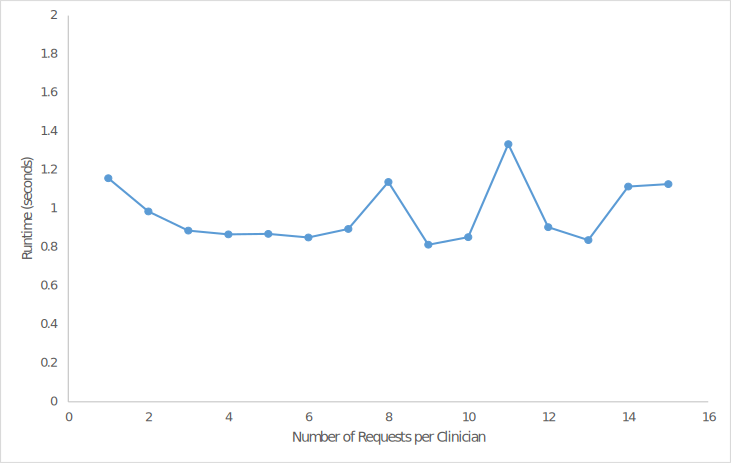
\includegraphics[scale=.5]{fig/runtime_requests}
	\caption{Runtime of ILP solver with an increasing number of requests per
		clinician}
	\label{fig:runtime-requests}
\end{figure}

Figure \ref{fig:runtime-blocks} presents the change in runtime when increasing
the number of 2-week blocks $B = \{26, 52, 78, 104\}$ in a department with 10
clinicians offering two services. There does not seem to be a strong effect on
runtime when we lengthen the time-horizon of the schedule, and in fact the
solver was able to find an optimal schedule for all time horizons within 3
seconds. \\ % 'very reasonable amount of time" is vague. what is reasonable?
%better to give a range in value.

\begin{figure}[h]
	\centering
	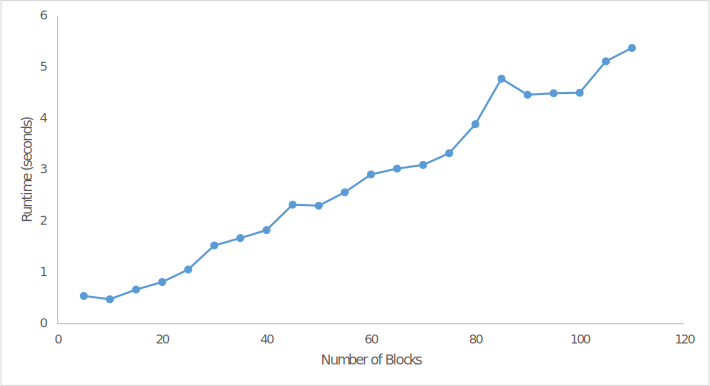
\includegraphics[scale=.5]{fig/runtime_blocks}
	\caption{Runtime of ILP solver with an increasing number of 2-week blocks}
	\label{fig:runtime-blocks}
\end{figure}

The effect of increasing the number of services %divisions %do you mean
%services?
on the runtime of the program is shown in Table
\ref{tbl:runtime-services-clinicians-comparison}. We executed the algorithm for
$S = \{1, 2, 3\}$ total services and $C = \{10, 20, 30, 50\}$ clinicians in
total across all services. For 2 concurrent services, a roster of 30 or more
clinicians becomes impractical to schedule, as searching for a solution required
over 24 hours. We saw similar issues for a roster of 20 or more clinicians
assigned to a division with 3 concurrent services. However, when relaxing the
NCB constraint, we saw a great improvement in runtime for divisions with 2 and 3
services, and we were able to generate a schedule with upwards of 50 clinicians
in under 1.5 seconds. \\  %what does division mean? do you mean services?

\begin{table}[htbp]
	\centering
 	\caption{Comparison of program runtime (in seconds) for different numbers of services and total clinicians in the division.}%
  \label{tbl:runtime-services-clinicians-comparison}%
	\begin{tabular}{|c|c||c|c||c|c|}
		\toprule
		                                      &  \multicolumn{5}{c|}{Number of Services}  \\ \midrule
		\makecell[l]{Number of \\ Clinicians} &  1   &    2    & 2 (without NCB) &  3   & 3 (without NCB) \\ \midrule
		                 10                   & 0.16 &  0.74   &  0.16   & 1.40 &  0.23   \\ \hline
		                 20                   & 0.25 & 7468.86 &  0.32   &  --  &  0.43   \\ \hline
		                 30                   & 0.42 &    --   &  0.49   &  --  &  0.66   \\ \hline
		                 50                   & 0.62 &    --   &  0.82   &  --  &  1.14   \\ \bottomrule
	\end{tabular}\\[1em]
  \footnotesize\raggedright
  Notes:
  ``--'' indicates that no solution was found within 24 hours;
  ``without NCB'' indicates that the No Consecutive Blocks (NCB) constraint was removed.
\end{table}
